% This is LLNCS.DOC the documentation file of
% the LaTeX2e class from Springer-Verlag
% for Lecture Notes in Computer Science, version 2.4
%\documentclass{llncs}
\documentclass{IEEEtran}
\usepackage{graphicx}
\usepackage{graphics}
\usepackage{listings}  
\usepackage{array}
\usepackage{multirow}
\usepackage[table]{xcolor}
\usepackage{float}
\usepackage{array}
\usepackage{ragged2e}
\newcolumntype{P}[1]{>{\RaggedRight\hspace{0pt}}p{#1}}

\usepackage{etoolbox}
\makeatletter
\patchcmd{\@makecaption}
{\scshape}
{}
{}
{}
\makeatother

\lstdefinestyle{base}{
	language=C,
	emptylines=1,
	breaklines=true,
	basicstyle=\ttfamily\color{black},
	moredelim=**[is][\color{red}]{@}{@},
}

\def\tablename{Table}

\usepackage[justification=centering]{caption}

\newcommand{\squeezeup}{\vspace{-2.5mm}}
\newcommand\FIXME[1]{\textbf{FIXME: #1}}
%
\begin{document}

\onecolumn

\title{Online Source Code Reuse: A Case Study of Stackoverflow \textit{vs.~}Qualitas OSS}
\maketitle

\section*{Raw statistics}
The results of running 2 clone detectors: Simian and NiCad, to detect clones between 144,075 Stackoverflow fragments (Java accepted answers) and 63 open-source projects in Qualitas dataset is presented below. There are 2 tools selected: Simian and NiCad. They are configured using three different settings: default settings, settings from FSE'13 paper, and settings from CloPlag experiment. Full Simian's parameter names can be found from the footnote\footnote{Simian's parameters: iChar = ignoreCharacters, iCurlB = ignoreCurlyBraces, iId = ignoreIdentifiers, iIdC = ignoreIdentifierCase, iMod = ignoreModifiers \newline iStrC = ignoreStringCase, iStr = ignoreStrings, iSbtNm = ignoreSubtypeNames, bSqBrck=balanceSquareBrackets}.

Manual investigation of Simian's clone report showed that there were problematic fragments (6 for defaults, 0 for FSE'13, and 11 for CloPlag). These fragments generate false clone containing array initialisation. Hence, they were removed from the result set before analysis.

\begin{table*}[h]
	\centering
	\caption{Simian clone results}
	\label{t_simian_raw_results}
	\begin{tabular}{l|r|r|r|r|r|r|r|r|r|r|r|r}
		\hline
		\multirow{4}{*}{} 
		& \multicolumn{4}{c|}{Default settings} 
		& \multicolumn{4}{c|}{Default settings*} 
		& \multicolumn{4}{c}{FSE'13 settings} \\ \cline{2-13} % & \multicolumn{4}{c}{CloPlag settings} \\
		& \multicolumn{4}{c|}{threshold=6} 
		& \multicolumn{4}{c|}{threshold=6} 
		& \multicolumn{4}{c}{threshold=5}  \\  % & \multicolumn{4}{c}{threshold=5} \\
		& \multicolumn{4}{c|}{iCharC,iCurlB,iIdC,iMod,iStrC} &
		\multicolumn{4}{c|}{iCharC,iCurlB,iIdC,iMod,iStrC,bSqBrck} & \multicolumn{4}{c}{iCurlB,iId,iIdC,iStr,iChar,iSbtNm,bSqBrck} \\\cline{2-13}  %  & \multicolumn{4}{c}{iId} \\
		% \hline
		& Frag.~ & $C_{\mathrm{pairs}}$ & $C_{\mathrm{SLOC}}$ & $C_{\mathrm{\%}}$ 
		& Frag.~ & $C_{\mathrm{pairs}}$ & $C_{\mathrm{SLOC}}$ & $C_{\mathrm{\%}}$ 
		& Frag.~ & $C_{\mathrm{pairs}}$ & $C_{\mathrm{SLOC}}$ & $C_{\mathrm{\%}}$ \\ % & Frag.~ & $C_{\mathrm{pairs}}$ & $C_{\mathrm{SLOC}}$ & $C_{\mathrm{\%}}$ \\
		\hline
		Removed & 6 & -- & -- & -- & 0 & -- & -- & -- & 0 & -- & -- & -- \\ %& 11 & -- & -- & -- \\
		Total          & 647       & 24,802       & --         & --  & 3   & 10 & -- & -- &  152 & 7,289,272 & -- & --  \\ % & 26,699 & 24,9702,821 & -- & --  \\
		Mean           & --        & 38           & 7.53       & 0.27   & -- & 3.33 & 8 & 0.29 & -- & 47,956 & 4.76 & 0.27 \\ % & -- & 9,356 & 4.74 & 0.26 \\
		Std Dev.       & -- 		  & 87		& 3.87 & 0.22 & -- & 2.62 & 1.41 & 0.18 & -- & 433,467 & 0.93 & 0.18 \\ % & -- & 96,038	& 0.99 & 0.18 \\
		Max            & --       & 551         & 63          & 0.94  & -- & 7	& 10 & 0.54 & -- & 5,278,408 & 8 & 0.83 \\ % & -- & 7,837,204 & 28 & 0.94 \\
		Min            & --       & 1           & 5           & 0.01  & -- & 1 & 7 & 0.10 & -- & 1 & 4 & 0.01 \\ % & -- & 1 & 4 & 0.002 \\
		Median         & --       & 3           & 7           & 0.22  & -- & 2 & 7 & 0.24 & -- & 22.5 & 4 & 0.23 \\ % & -- & 27 & 4 & 0.22 \\
		Mode           & --       & 1           & 7           & 0.25  & -- & N/A & 7 & N/A & -- & 1 & 4 & 0.50 \\ % & -- & 1 & 4 & 0.50 \\
		\hline
	\end{tabular} 
\end{table*}

\begin{table*}[h]
	\centering
	\caption{NiCad clone results}
	\label{t_nicad_raw_results}
		\begin{tabular}{l|r|r|r|r|r|r|r|r}
			\hline
			\multirow{4}{*}{} & \multicolumn{4}{c|}{Default settings} & \multicolumn{4}{c}{FSE'13 settings} \\ \cline{2-9} 
			%& \multicolumn{4}{c|}{Default settings} & \multicolumn{4}{c|}{FSE'13 settings}  & \multicolumn{4}{c}{CloPlag settings} \\
			%\hline
			& \multicolumn{4}{c|}{threshold=6, UPI=0.30} & \multicolumn{4}{c}{threshold=5, UPI=0.2} \\ % & \multicolumn{4}{c}{threshold=6, UPI=0.4} \\
			& \multicolumn{4}{c|}{rename=none,abstract=none} & \multicolumn{4}{c}{rename=blind,abstract=literal} \\ \cline{2-9} % & \multicolumn{4}{c}{rename=blind,abstract=declaration} \\
			%\hline
			& Frag.~ & $C_{\mathrm{pairs}}$ & $C_{\mathrm{SLOC}}$ & $C_{\mathrm{\%}}$ & Frag.~ & $C_{\mathrm{pairs}}$ & $C_{\mathrm{SLOC}}$ & $C_{\mathrm{\%}}$ \\ % & Frag.~ & $C_{\mathrm{pairs}}$ & $C_{\mathrm{SLOC}}$ & $C_{\mathrm{\%}}$ \\
			\hline
			Total & 983 & 106,091 & -- & -- & 8,100 & 31,141,599 & -- & --    \\
			Mean & -- & 108 & 9.48 & 0.25 & -- & 3,845 & 5.52 & 0.19 \\
			Std Dev. & 	& 200.49 & 3.04	& 0.18 & -- & 4,305 & 2.49 & 0.15 \\
			Max & -- & 1816 & 39 & 0.80 & -- & 46,469 & 111 & 0.88 \\
			Min & -- & 1 & 7 & 0.02 & -- & 1 & 3	 & 0.01 \\
			Median & -- & 14 & 8 & 0.19 & -- & 3,095 & 5 & 0.14 \\
			Mode & -- & 1 & 8 & 0.53 & -- & 1 & 4 & 0.33 \\
			\hline
		\end{tabular} 
\end{table*}

%\section*{Agreed Cloned Fragments}
%The results from both tools are compared to find clone pairs that they mutually agree.  Theses agreed clone pairs will be manually investigated. The results of agreed clone pairs found by different parameter settings of Simian and NiCad are shown in Table \ref{t_agreed_clone}.

%\begin{table}[h]
%	\centering
%	\caption{Agreed cloned fragments between Simian and Nicad}
%	\label{t_agreed_clone}
%	\begin{tabular}{l|r|r}
%		\hline
%		& Simian$_{\mathrm{\textit{default}}}$ & Simian$_{\mathrm{\textit{fse13}}}$ \\ % & Simian$_{\mathrm{\textit{cloplag}}}$ \\
%		\hline
%		NiCad$_{\mathrm{\textit{default}}}$ & 92          & 1        \\%      & 709             \\
%		NiCad$_{\mathrm{\textit{fse13}}}$   & 155         & 25           \\ % & 4680            \\
		%NiCad$_{\mathrm{\textit{cloplag}}}$ &             &               \\ % &                \\
%		\hline
%	\end{tabular}
%\end{table}

%Relationships between the cloned fragments are displayed in Fig.~\ref{fig:venn4}.

%\begin{figure}[H]
%\centering
%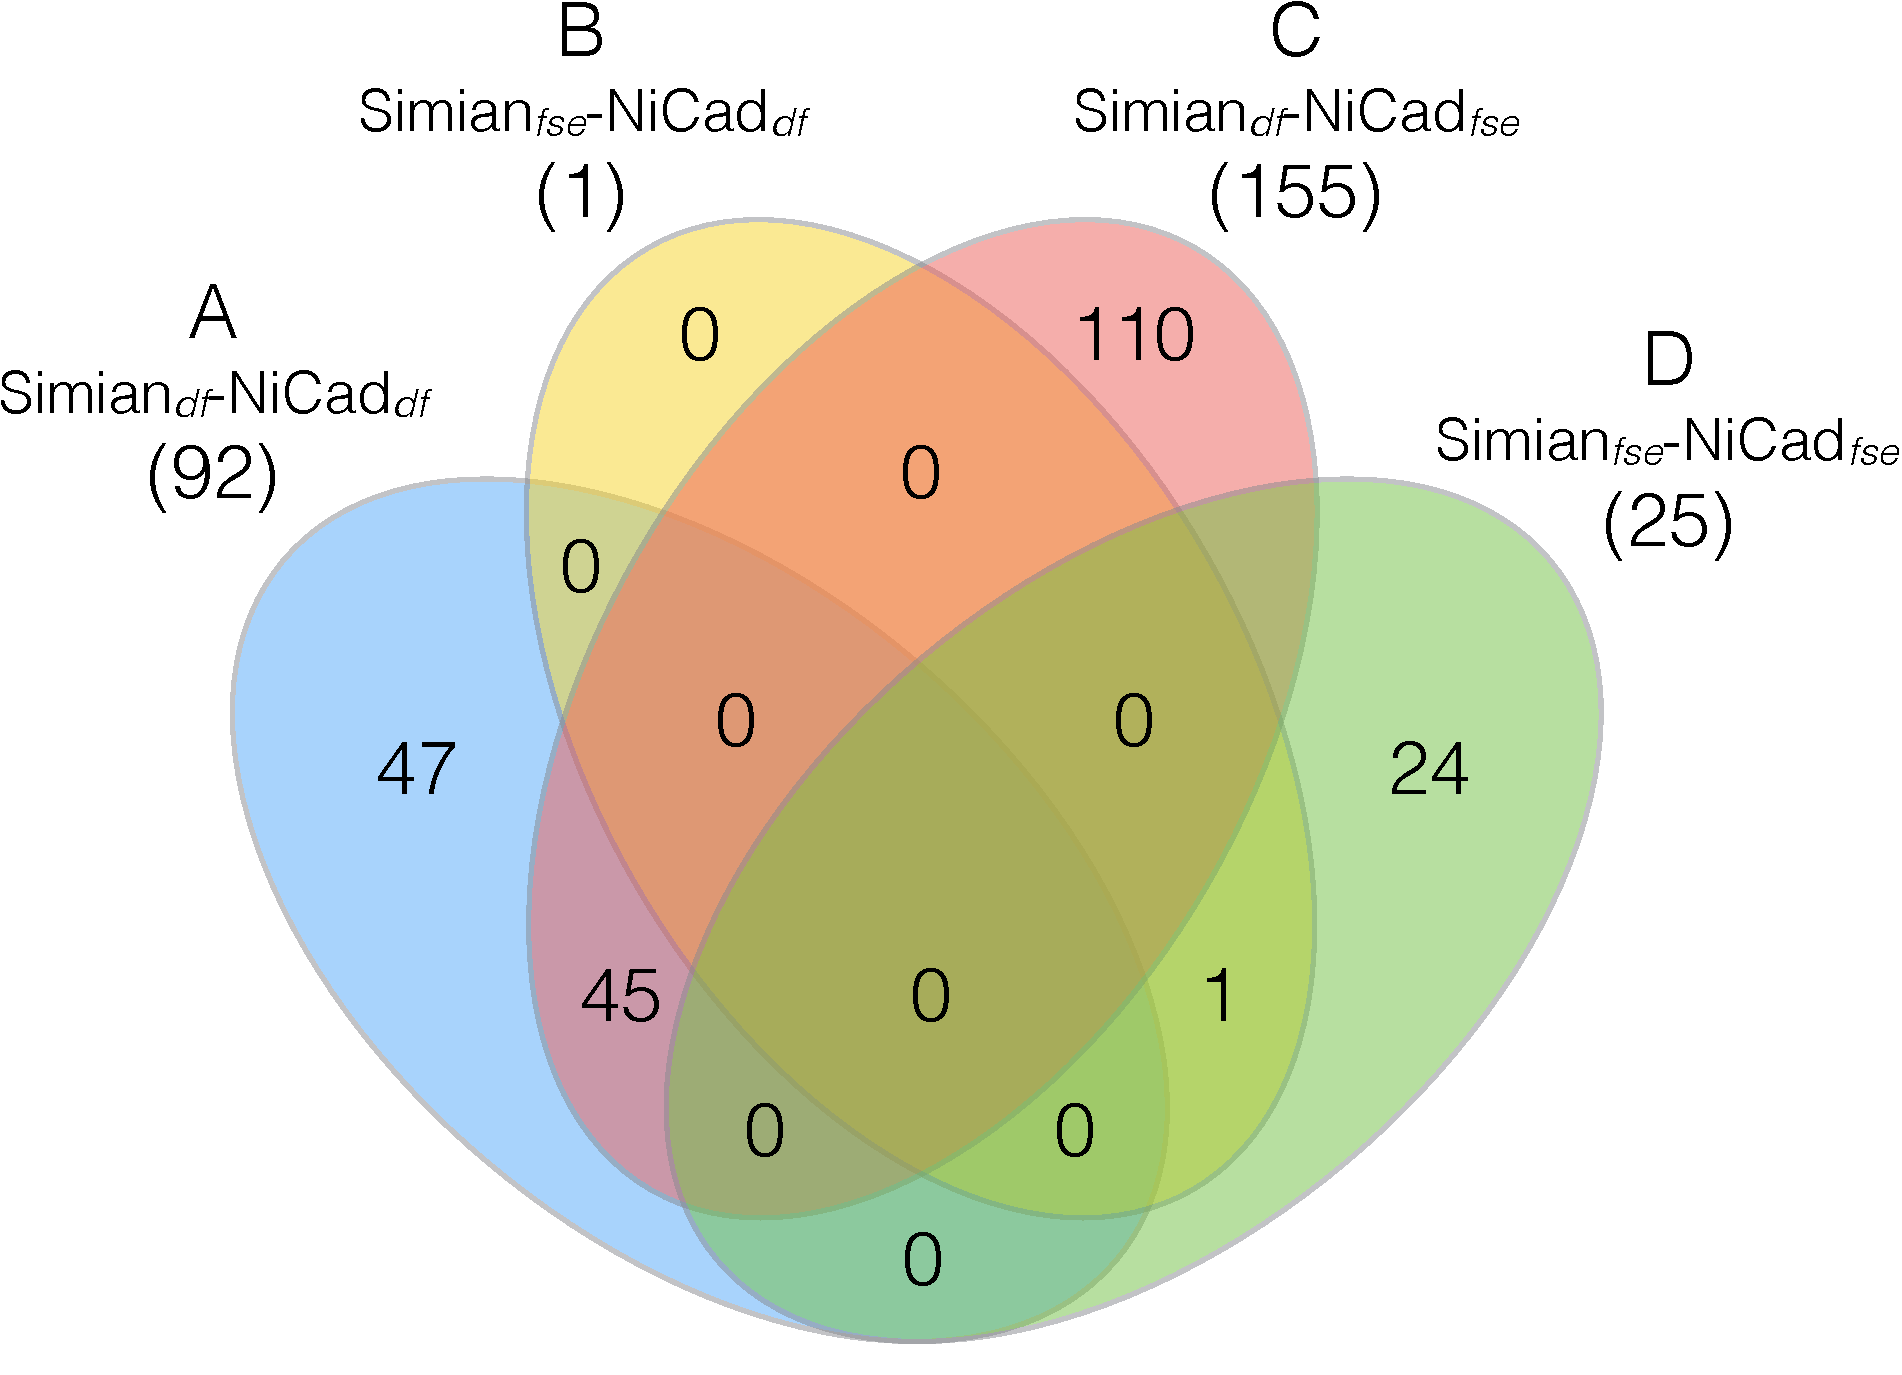
\includegraphics[width=0.5\linewidth]{venn4}
%\caption[Agreed clone fragments reported by Simian and NiCad with default and FSE'13 settings]{Agreed clone fragments reported by Simian and NiCad with default and FSE'13 settings}
%\label{fig:venn4}
%\end{figure}

\section*{Agreed Clone Pairs}
The investigation of the clone pairs using Bellon's \textit{good-match(p)} and \textit{ok-match(p)} criteria are listed in  Table \ref{t_agreed_good_clone_pairs} and Table \ref{t_agreed_ok_clone_pairs}. We use the threshold \textit{p} of 0.7 for both \textit{good-match} and \textit{ok-match}. Visualisation of \textit{good-match} common clone pairs between sets of parameter settings can be seen from Figure \ref{fig:venn4_pairs}. There are 14 \textit{good-match} pairs. The \textit{ok-match} subsumes the \textit{good-match} resulting in totally 528 common clone pairs.

\begin{table}[h]
	\centering
	\caption{18 agreed good-match(0.7) cloned pairs between Simian and Nicad (14 are unique)}
	\label{t_agreed_good_clone_pairs}
	\begin{tabular}{l|r|r}
		\hline
		& Simian$_{\mathrm{\textit{default}}}$ & Simian$_{\mathrm{\textit{fse13}}}$ \\ % & Simian$_{\mathrm{\textit{cloplag}}}$ \\
		\hline
		NiCad$_{\mathrm{\textit{default}}}$ & 9 & 1 \\ %      & 709             \\
		NiCad$_{\mathrm{\textit{fse13}}}$   & 3 & 5 \\ % & 4680            \\
		%NiCad$_{\mathrm{\textit{cloplag}}}$ &             &               \\ % &                \\
		\hline
	\end{tabular}
\end{table}

\begin{table}[H]
	\centering
	\caption{Duplicated agreed \textit{good}-pairs between pairs of Simian and NiCad settings}
	\label{t_dup_agreed_good_clone_pairs}
	\begin{tabular}{l|r|r|r|r}
		\hline
		& $S_dN_d$ & $S_dN_f$ & $S_fN_d$ & $S_fN_f$ \\ % & Simian$_{\mathrm{\textit{cloplag}}}$ \\
		\hline
		$S_dN_d$ & 9 & 3 & 0 & 0 \\%      & 709             \\
		$S_dN_f$ & 3 & 3 & 0 & 0 \\ % & 4680            \\
		$S_fN_d$ & 0 & 0 & 1 & 1 \\
		$S_fN_f$ & 0 & 0 & 1 & 5 \\	
		%NiCad$_{\mathrm{\textit{cloplag}}}$ &             &               \\ % &                \\
		\hline
	\end{tabular}
\end{table}

\begin{figure}[H]
	\centering
	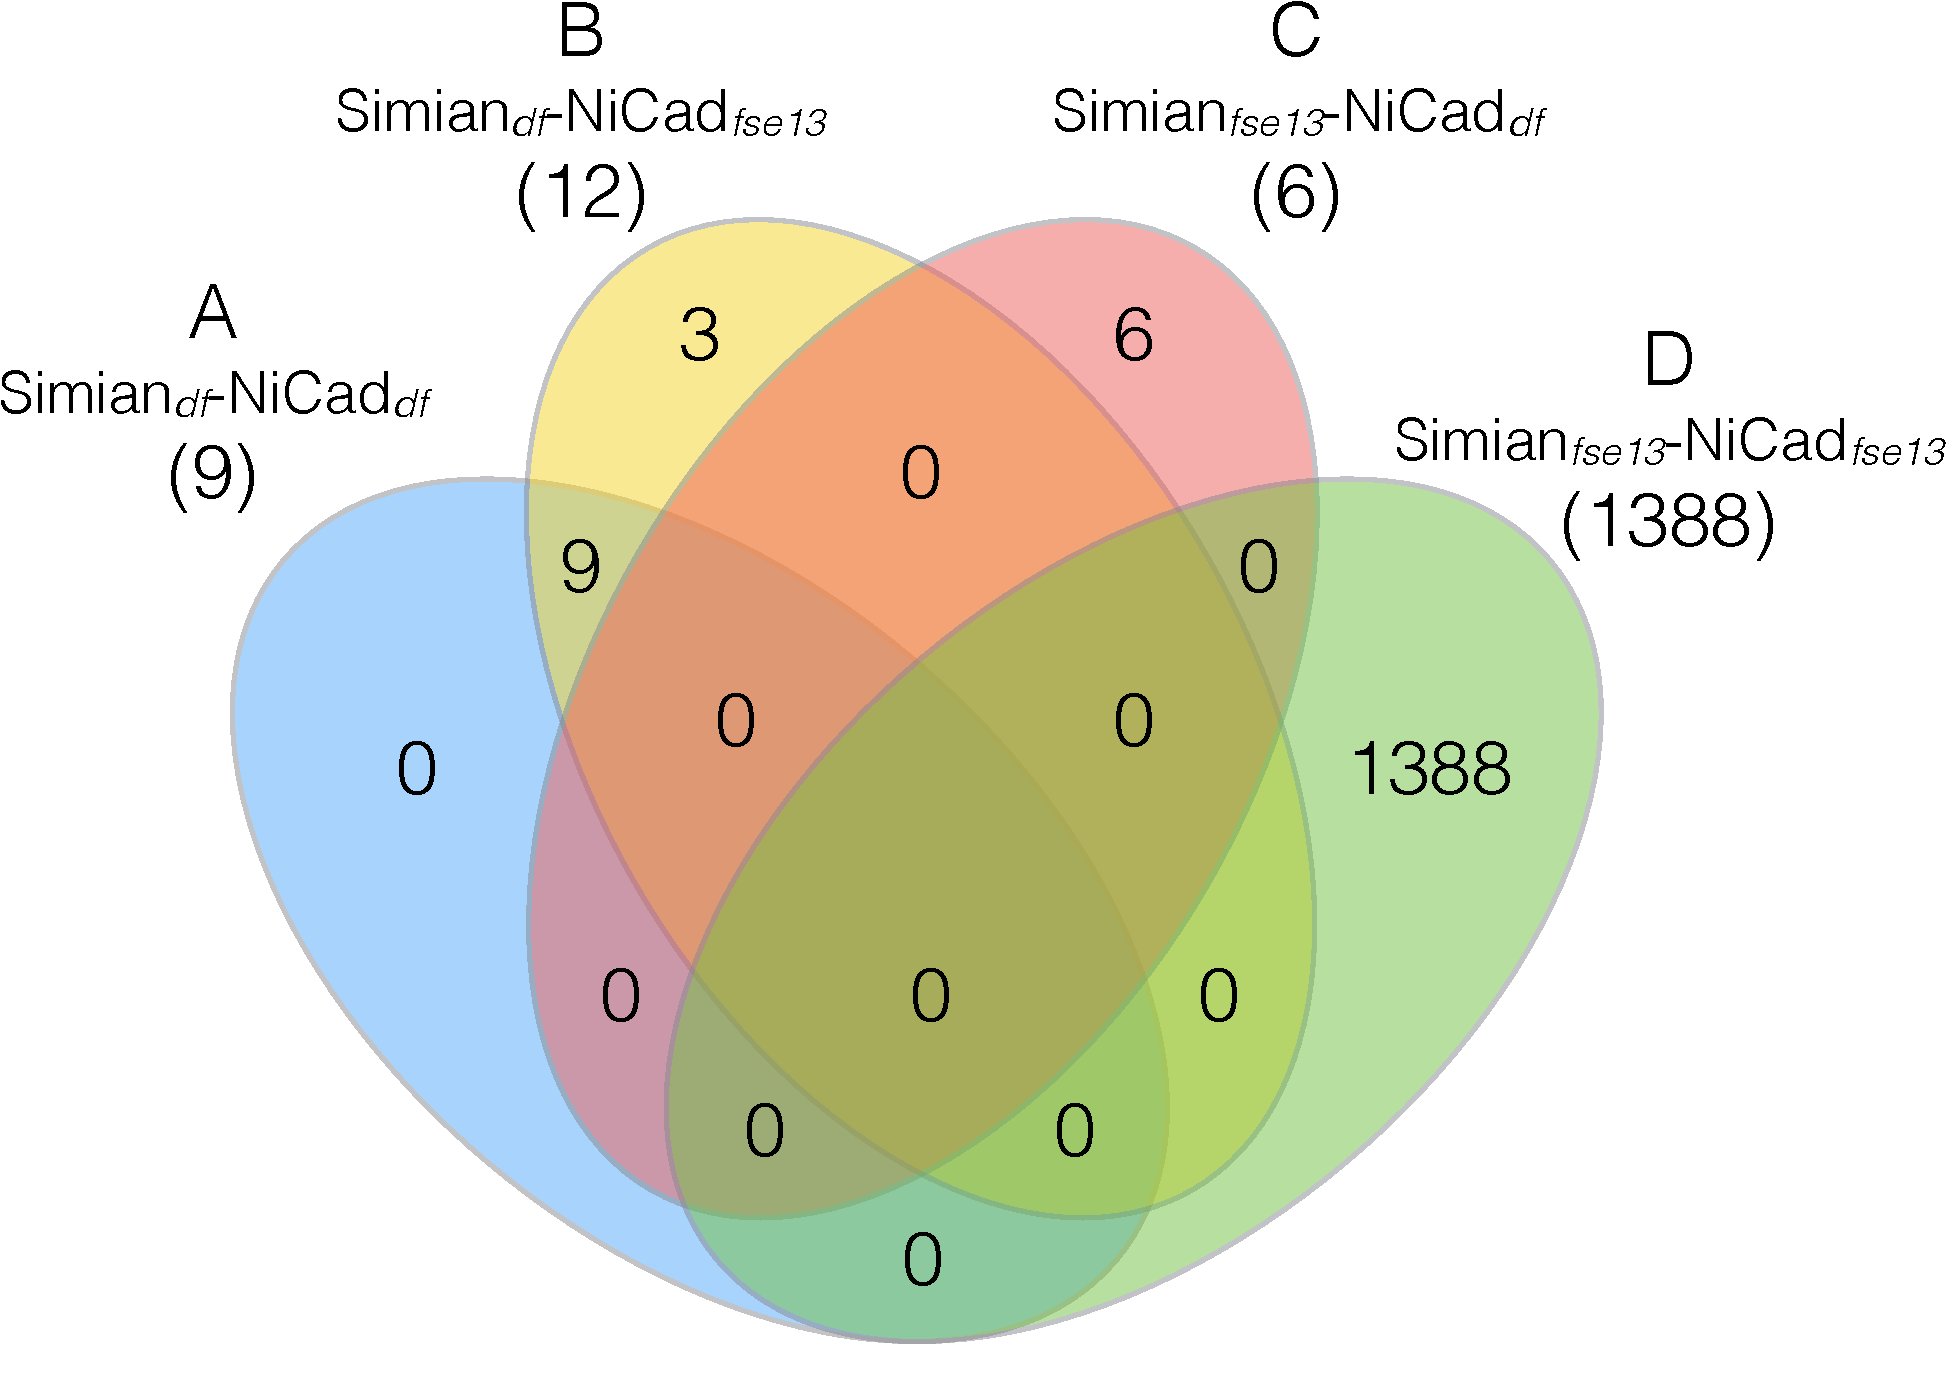
\includegraphics[width=0.5\linewidth]{venn4_pairs_good}
	\caption[Agreed clone pairs reported by Simian and NiCad with default and FSE'13 settings using good-match(0.7) criterion]{Agreed clone pairs reported by Simian and NiCad with default and FSE'13 settings using good-match(0.7) criterion}
	\label{fig:venn4_pairs}
\end{figure}

\begin{table}[h]
	\centering
	\caption{528 agreed ok-match(0.7) cloned pairs between Simian and Nicad (510 are unique)}
	\label{t_agreed_ok_clone_pairs}
	\begin{tabular}{l|r|r}
		\hline
		& Simian$_{\mathrm{\textit{default}}}$ & Simian$_{\mathrm{\textit{fse13}}}$ \\ % & Simian$_{\mathrm{\textit{cloplag}}}$ \\
		\hline
		NiCad$_{\mathrm{\textit{default}}}$ & 373 & 1 \\%      & 709             \\
		NiCad$_{\mathrm{\textit{fse13}}}$   & 118 & 36 \\ % & 4680            \\
		%NiCad$_{\mathrm{\textit{cloplag}}}$ &             &               \\ % &                \\
		\hline
	\end{tabular}
\end{table}

\begin{table}[h]
	\centering
	\caption{Duplicated agreed \textit{ok}-pairs between Simian and NiCad settings  (510 are unique)}
	\label{t_dup_agreed_ok_clone_pairs}
	\begin{tabular}{l|r|r|r|r}
		\hline
		& $S_dN_d$ & $S_dN_f$ & $S_fN_d$ & $S_fN_f$ \\ % & Simian$_{\mathrm{\textit{cloplag}}}$ \\
		\hline
		$S_dN_d$ & 373 & 17 & 0 & 0 \\%      & 709             \\
		$S_dN_f$ & 17 & 118 & 0 & 0 \\ % & 4680            \\
		$S_fN_d$ & 0 & 0 & 1 & 1 \\
		$S_fN_f$ & 0 & 0 & 1 & 36 \\	
		%NiCad$_{\mathrm{\textit{cloplag}}}$ &             &               \\ % &                \\
		\hline
	\end{tabular}
\end{table}

\begin{figure}[H]
	\centering
	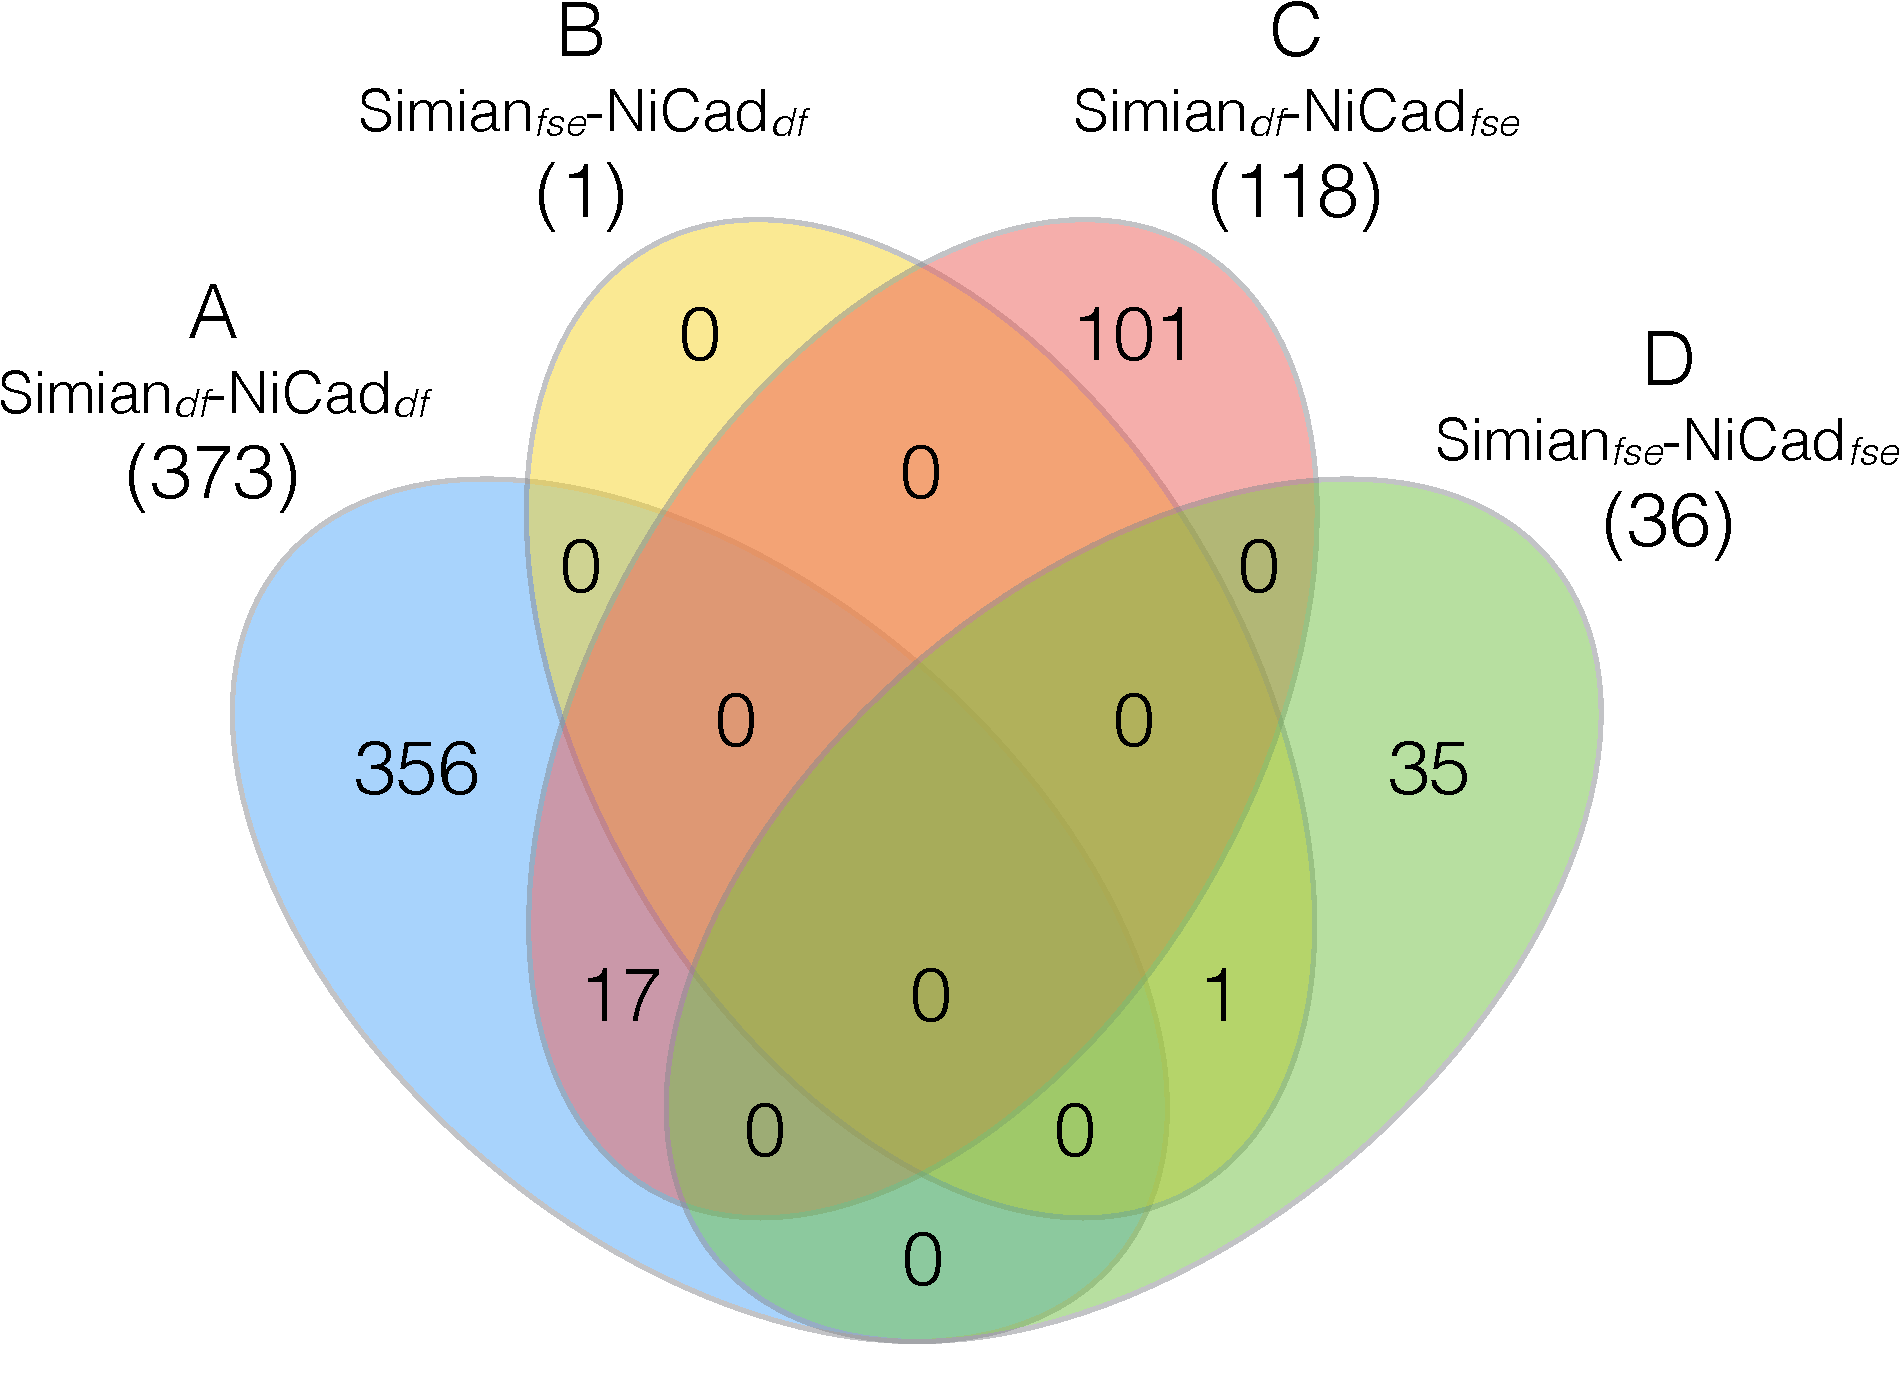
\includegraphics[width=0.5\linewidth]{venn4_pairs_ok}
	\caption[Agreed clone pairs reported by Simian and NiCad with default and FSE'13 settings using ok-match(0.7) criterion]{Agreed clone pairs reported by Simian and NiCad with default and FSE'13 settings using ok-match(0.7) criterion}
	\label{fig:venn4_pairs}
\end{figure}

\section*{Investigation of Missing A/B Clone Pairs Reported by Simian (df)}
We investigated the 41 clone pairs previously reported by Simian with default configurations and manually investigated. The 41 pairs were searched for in 4 new results sets: Simian$_{df}$, Simian$_{fse13}$, NiCad$_{df}$, NiCad$_{fse13}$. The investigation results are shown in Table \ref{tab:search}.

\begin{table}[H]
	\centering
	\caption{Results of matching the original 41 Simian(default) pairs in the pretty-printed result sets}
	\label{tab:search}
	\begin{tabular}{l|r|r}
		\hline 
		Settings & Found & Not found \\ 
		\hline 
		Simian$_{df}$  &  40 & 1* \\ 
		\hline 
		Simian$_{fse13}$ & 0 & 41  \\ 
		\hline 
		NiCad$_{df}$  & 9 & 32 \\ 
		\hline 
		NiCad$_{fse13}$ &  9 & 32 \\ 
		\hline 
	\end{tabular} 
\end{table}

The single missing Stackoverflow fragment (19051537\_0.java) (denoted by *) is one of the 6 false clones generated by Simian. It is removed from the results of the pretty-printed version because it is an outlier. The rest are missing because of different parameter settings.


\section*{Manual Investigation}

\subsection{Investigation of agreed \textit{good} and \textit{ok}-match clone pairs}
I have manually investigated all of the 14 \textit{good-match} ones and 510 \textit{ok-match} ones. The classification schems is described in Table \ref{tab:classification_scheme} and the classification results are shown in Table \ref{tab:classification}. 

Since we are not certain about the direction of copying in the B-classified pairs, we checked the modification time of each Java file in Qualitas project and compare it to the timestamp of Stackoverflow answers. We found that all Stackoverflow code fragments were posted after their respectively similar Java files in Qualitas project. This means that the copying can only be either (1) S $\leftarrow$ Q or (2) from a third source to both S and Q independently.

\subsection{Investigation of extra 100 clone pairs}
In the preliminary stage of our experiment, we found that there are 41 Stackoverflow fragments reported by Simian with default configurations. However, only 10 of them appear in the new results using tool's agreement. Thus, we further investigated the clone pairs reported by Simian and NiCad but \textit{without} an agreement. With our 4 settings, we investigated the largest 25 clone pairs (according to their average SLOC) resulting in 100 more manually investigated pairs. The classification results are shown in Table \ref{tab:classification} and Table \ref{tab:classification_breakdown}.


\begin{table}[H]
	\centering
	\caption{Classification results of 14 \textit{good} and 510 \textit{ok}-matches (including the subsumed \textit{good}-match pairs).}
	\label{tab:classification}
	\begin{tabular}{|l|r|r|r|r|r|r|r|}
		\hline 
		Classification & A & B & C & D & E & F & Total \\ 
		\hline 
		\multirow{2}{*}{\textit{good-match(0.7)}} & 1 & 2 & 2 & 2 & 7 & 0 & 14 \\ \cline{2-8}
		& 7.14\%	& 14.29\%	& 14.29\%	& 14.29\%	& 50.00\%	& 0.00\%	& 100.00\% \\ 
		\hline
		\multirow{2}{*}{\textit{ok-match(0.7)}} & 4 & 42 & 8 & 351 & 28 & 77 & 510 \\ \cline{2-8}
		& 0.78\%	& 8.24\%	&	1.57\%	&	68.82\%	&	5.49\%	&	15.10\%	&	100.00\%  \\ 
		\hline
		\multirow{2}{*}{100 indv. pairs} & 12 & 6 & 1 & 18 & 1 & 62 & 100 \\ \cline{2-8}
		& 12\%	& 6\%	&	1\%	&	18\%	&	1\%	&	62\%	&	100\%  \\ 
		\hline
	\end{tabular} 
\end{table}

\begin{table}[H]
	\centering
	\caption{Breakdowns of 100 individual clone pairs}
	\label{tab:classification_breakdown}
	\begin{tabular}{|l|r|r|r|r|r|r|r|}
		\hline 
		Classification & A & B & C & D & E & F & Total \\ 
		\hline 
		Simian$_df$ & 12 & 6 & 1 & 2 & 0 & 4 & 25 \\ 
		\hline
		Simian$_fse13$ & 0 & 0 & 0 & 0 & 0 & 25 & 25 \\
		\hline
		NiCad$_df$ & 0 & 0 & 0 & 11 & 0 & 14 & 25 \\
		\hline
		NiCad$_fse13$ & 0 & 0 & 0 & 5 & 1 & 19 & 25 \\
		\hline
		Total & 12 & 6 & 1 & 18 & 1 & 62 & 100 \\
		\hline
	\end{tabular} 
\end{table}

\begin{table}[H]
	\centering
	\caption{Classifications of clone creation}
	\label{tab:classification_scheme}
	\begin{tabular}{|c|p{13cm}|}
		\hline 
		Category & Descriptions \\ 
		\hline 
		A & Code in Stackoverflow is copied from Qualitas (S $\leftarrow$ Q). \\ 
		\hline 
		B & Code is copied either from each other or a third source (unknown) (S $\leftrightarrow$ Q).
		\\ 
		\hline 
		C & Code in both places are copied from a third source T (known) (S, Q $\leftarrow$ T ).
		\\ 
		\hline 
		D & Code is a boiler-plate or IDE auto-generated.
		\\ 
		\hline 
		E & Code in both places initialise a similar/the same object; extend the same class/its subclass; implement the same interface.
		\\ 
		\hline 
		F & Accidental similarity  \\ 
		\hline 
	\end{tabular} 
\end{table}

\newpage

\section*{Simian's Parameters}

We have carefully investigated the effects of the Simian's parameter \texttt{-balanceSquareBrackets+}. I found that it works in the expected way of handling a pair of brackets (\texttt{[},\texttt{]}) that span over multiple lines. For example, the two code fragments in Figure \ref{fig:two_frags} would match by having \texttt{-balanceSquareBrackets+} enabled.

\noindent\begin{figure}[H]
	\scriptsize
	\begin{lstlisting}[frame=single,style=base]
1           public class MagicSquare {                             public class MagicSquare2 {
2               private int[][] square;                                @private int[@
3               private boolean[] possible;                                        @][@
4               private int totalSqs;                                              @] square;@
5               private int sum;                                       private boolean[] possible;
6               private int numsquares;                                private int totalSqs;
7               public static void main ( String[] args ) {            private int sum;
8               MagicSquare m = new MagicSquare ( 3 );                 private int numsquares;
9                                                                      public static void main ( String[] args ) {
10                                                                     MagicSquare m = new MagicSquare ( 3 );
	\end{lstlisting}
	\caption{Two identical fragments with only differences in locations of the square brackets. All 7 lines are reported by Simian if \small\texttt{-balanceSquareBrackets+} \normalsize is enabled. If not, the clone pairs is reported as \newline (MagicSquare.java [3,8], MagicSquare2.java [5,10]).} 
	\label{fig:two_frags}
\end{figure}

However, the -balanceSquareBrackets+ parameter only works on a small testing environment having toy programs or only small pairs from the full datasets. It does not work with the full complete set of 144,075 Stackoverflow fragments and Qualitas projects. Please find the summary of all the testing scenarios in Table \ref{tab:summary}. %I found that this pair is missing if I turned on \texttt{-balanceSquareBrackets+}.

\begin{table}[H]
	\caption{Simian's \texttt{-balanceSquareBrackets+} (\texttt{-bsb+}) is observed to have unpredictable behaviours when running against big datasets. $\textrm{\textit{CP}}_2$ means the reported clone(s) do not contain lines having dislocated brackets ($L_b$) (i.e. $\textrm{\textit{CP}}_2 = \textrm{\textit{CP}}_1 - L_b$).}
	\label{tab:summary}
	\centering
	\small\begin{tabular}{l|p{6cm}|c|c|c}
		\hline 
		\multirow{2}{*}{\textbf{Project 1}} & \multirow{2}{*}{\textbf{Project 2}} & \textbf{Dislocated} & \multirow{2}{*}{\textbf{-bsb+}} & \textbf{Clones pair} \\ 
		& & \textbf{brackets?} & & \textbf{reported} \\
		\hline
		\hline
		\multicolumn{5}{l}{\textit{Only run Simian against the pair}} \\
		\hline
		MagicSquare.java & MagicSquare\_exact\_copy.java & no & 0,1 & $\textrm{\textit{CP}}_1$ \\
		MagicSquare.java & MagicSquare2.java & yes & 0 & $\textrm{\textit{CP}}_2$ \\ 
		MagicSquare.java & MagicSquare2.java & yes & 1 & $\textrm{\textit{CP}}_1$ \\
		\hline
		%\hline
		%\multicolumn{5}{c}{\textit{Only run Simian against the pair}} \\
		%\hline
		stackoverflow/4298836\_0.java & Qualitas/aoisrc281/../ExprModule.java & no & 0 & $\textrm{\textit{CP}}_3$ \\ 
		stackoverflow/4298836\_0.java & Qualitas/aoisrc281/../ExprModule.java & no & 1 & $\textrm{\textit{CP}}_3$ \\ 
		stackoverflow/4533682\_1.java & Qualitas/cobertura-1/../TouchCollector.java & no & 0 & $\textrm{\textit{CP}}_4$ \\ 
		stackoverflow/4533682\_1.java & Qualitas/cobertura-1/../TouchCollector.java & no & 1 & $\textrm{\textit{CP}}_4$ \\ 
		\hline 
		\hline
		\multicolumn{5}{l}{\textit{Run Simian against the complete stackoverflow data and the project}} \\
		\hline
		stackoverflow/4298836\_0.java & Qualitas/aoisrc281/../ExprModule.java & no & 0 & $\textrm{\textit{CP}}_3$ \\ 
		\cellcolor{red!10}stackoverflow/4298836\_0.java & \cellcolor{red!10}Qualitas/aoisrc281/../ExprModule.java & \cellcolor{red!10}no & \cellcolor{red!10}1 & \cellcolor{red!10}-- \\ 
		\hline
		stackoverflow/4533682\_1.java & Qualitas/cobertura-1/../TouchCollector.java & no & 0 & $\textrm{\textit{CP}}_4$ \\ 
		\cellcolor{red!10}stackoverflow/4533682\_1.java & \cellcolor{red!10}Qualitas/cobertura-1/../TouchCollector.java & \cellcolor{red!10}no & \cellcolor{red!10}1 & \cellcolor{red!10}-- \\
		\hline 
	\end{tabular} 
\end{table}

\end{document}
